\documentclass[referee, 
	            sn-basic]
           {sn-jnl}

\usepackage{lineno,hyperref}
\usepackage{longtable, booktabs, amsmath, textcomp}
\usepackage{natbib}

% Put Abstract on new page to create title page as per Oecologia guidelines
	\usepackage{etoolbox}
	\pretocmd{\abstractname}{\newpage}{}{}

% Springer stuff 
\jyear{2022}%
\raggedbottom
\unnumbered% uncomment for unnumbered level heads

\begin{document}
\raggedright

\title[Rangeland grasshoppers and prescribed fire]{Attracted by higher crude protein, grasshopper abundance and offtake increase after prescribed fire\footnote{Author contributions:
NGH collected data. 
NGH and DAM analyzed data. 
NGH wrote the initial draft of the paper, which DAM and CLW edited with input from LV and DB.
LV was responsible for the prescribed fire treatments from which data were collected. 
DB provided grasshopper expertise and sampling equipment. }}


\author*[1]{\fnm{Nicholas Gregory}  \sur{Heimbuch}}\email{ngh11@pitt.edu}

\author[2]{\fnm{Devan Allen} \sur{ McGranahan}}\email{Devan.McGranahan@usda.gov}
\author[3]{\fnm{Carissa L.} \sur{ Wonkka}}\email{Carissa.Wonkka@usda.gov }
\author[2]{\fnm{Lance} \sur{Vermiere}}\email{Lance.Vermiere@usda.gov}
\author[3]{\fnm{David} \sur{Branson}}\email{David.Branson@usda.gov }

\affil*[1]{\orgname{University of Pittsburg}, 
	     \orgdiv{ },
              \orgaddress{\street{ }, 
            		     \city{Pittsburg},
            		     \postcode{ }, 
           		     \state{Pennsylvania},
            		     \country{USA}}}

\affil[2]{\orgname{USDA Agricultural Research Service}, 
	     \orgdiv{Livestock \& Range Research Laboratory},
              \orgaddress{\street{243 Ft. Keogh Rd.}, 
            		     \city{Miles City},
            		     \postcode{59301}, 
           		     \state{Montana},
            		     \country{USA}}}
\affil[3]{\orgname{USDA Agricultural Research Service}, 
	     \orgdiv{Northern Plains Agricultural Research Laboratory},
              \orgaddress{\street{1500 N Central Ave}, 
            		     \city{Sidney},
            		     \postcode{59270}, 
           		     \state{Montana},
            		     \country{USA}}}
        

           		     
\clearpage

\abstract{Little research has been done to examine the influences of fire and drought on grasshopper herbivory patterns. 
Climate warming is producing more frequent and more intense droughts in the Northern Great Plains region of the United States, affecting herbivore resource availability and stressing the range ecosystem. 
This study created three different time since fire treatments to examine how indirect fire effects (improved forage quality) affect the density and offtake of local grasshoppers.
Both offtake and density were significantly higher in burned locations compared to unburned control plots. 
Burned plot grasshopper density increased greatly over time, while density remained constant in unburned locations. 
These density patterns appear to be the direct result of the high protein content found in burned locations. 
The results raise further questions into the mechanism that produces the magnet effect in range grasshoppers. 
These results also highlight the importance of understanding how fire will interact with future climate conditions to affect range herbivore interactions.} 
\keywords{prescribed fire; }

\maketitle
\begin{linenumbers}

\section{Introduction}

As globally-ubiquitous herbivores, grasshoppers (Orthoptera: Acrididae) contribute to ecosystem function around the world. 
Historically, interest in grasshoppers has generally increased with their local density, as grasshopper outbreaks and locust swarms have wrought economic damage for centuries \citep{cease2015}. 
While such outbreaks were long considered to be primarily driven by environmental conditions beyond human control, research has described close interactions between land management and grasshopper dynamics \citep{legall2019}. 
Although the utility of this broader understanding of grasshoppers and human land use has mostly been realized within the context of pest control \citep{branson2006}, grasshoppers also contribute to ecosystem dynamics including nutrient cycling and plant community composition \citep{meyer2002,zhang2011,kietzka2021}. 

Grasshoppers are particularly important in \emph{open ecosystems}\textemdash rangeland biomes such as grasslands and savannas characterized by dominant herbaceous communities regulated by frequent disturbances, including herbivory and fire \citep{bond2022}. 
There are myriad interactions between grasshoppers, fire, and, particularly, other herbivores. 
Grasshoppers are widely seen as pests in competition with economically-valuable livestock for herbaceous primary productivity \citep{zhang2019a}. 
For example, \citet{hewitt1983} estimated grasshoppers consume nearly US\$400 million worth of livestock forage per year in the western United States. 
Meanwhile, fire interacts with grasshoppers via direct and indirect effects, which are variable among species depending on their biology \citep[e.g.][]{vermeire2004}. 
Direct effects include mortality of adults and eggs from heat exposure, while indirect effects include alterations to host plant availability, vegetation structure, and microclimate. 

Because the nutritive value of vegetation in open ecosystems often varies depending on the time since it last burned, fire likely also affects grasshoppers by modulating their food resources. 
Perennial, fire-adapted plants resprout using energy stored in organs protected from heat damage, and post-fire plant tissue is typically higher in crude protein and lower in structural carbohydrates than the mature or senescent tissue that was consumed by the fire \citep{mcgranahan2021}. 
Thus, despite overall lower plant biomass on account of the fire, grasshopper abundance on recently-burned areas is often higher than unburned areas, especially for graminivorous  (grass-eating) species \citep{meyer2002}. 
More broadly, post-disturbance succession and plant nutritive value have been identified as important factors in grasshopper abundance \citep{fartmann2012, schirmel2019}. 
But explicit examinations between time-since-fire, plant nutritive value, and grasshopper abundance have yet to be conducted. 

We measured grasshopper abundance and forage consumption, along with grass protein content, in a replicated experiment that created a time-since-fire gradient in temperate grassland.  
Because grasshoppers are morphologically capable of much more precise herbivory than most vertebrate grazers, we measured protein content of grass leaves and stems separately.
We predicted that more-recently burned plots would have both higher protein content\textemdash especially in leaves\textemdash and greater grasshopper abundance. 
As such, we predicted a greater degree of vegetation removal by grasshoppers from recently-burned plots, as determined by comparing aboveground plant biomass against that from within grasshopper exclosures. 

\section{Methods}

\subsection{Study location \& design} 

Our study was conducted at the USDA-Agricultural Research Service Livestock and Range Research Station in Miles City, Montana, USA (46.40 N, 105.95 W).  
Vegetation is typical mixed-grass prairie, and the study site was dominated by western wheatgrass \emph{Pascopyrum smithii}.  
The overwhelming majority of grasshoppers on the study site, as determined by mid-season sweep netting and identification at the USDA-ARS Pest Management Research Unit in Sidney, Montana, were the migratory grasshopper \emph{Melanoplus sanguinipes}, a native species of spur-throated grasshopper in the family Acrididae. 

Within a larger prescribed fire experiment, we selected nine, 375-m\textsuperscript{2} plots to test three different time-since-fire treatments (n=3 each): Fire the previous autumn, fire the previous spring, and a control treatment left unburned for several years. 
Livestock were excluded from the entire study area and had been for several years.
While the study area was open to wildlife such as deer \emph{Odocoileus} spp., pronghorn \emph{Antilocapra americana}, and lagomorphs including \emph{Sylvilagus floridanus} and \emph{Lepus} spp, we observed no evidence of their presence on any plots during the sampling period. 

\subsection{Sample collection}

To measure the amount of vegetation removed by foraging grasshoppers, we established two pairs of sample points within each plot. 
Each pair of 0.25-m\textsuperscript{2} sample points consisted of one full mesh grasshopper exclosure alongside another structure with a similar footprint and shade factor that was open to grasshopper herbivory.
Each type of structure consisted of a polyvinyl chloride tube frame with heavy nylon netting, which when fully wrapped and zipped around the frame and weighted down with sand-filled tubes, effectively kept grasshoppers out \citep{parker1985}. 
Because the mesh reduced sunlight intensity by 400 w m\textsuperscript{-2} compared to the
surrounding area, we designed control structures that remain open on the north and south faces to allow grasshoppers to enter while still producing shade conditions that matched the exclosures during peak photosynthesis hours. 
These paired structures ensured that shade would not influence grass development and skew our offtake measurements. 
Structures were monitored at least every 48 hr and after any substantial weather event to ensure they remained intact; in the few instances grasshoppers had crawled under the exclosures, they were removed upon discovery. 

On all plots, the first pair of structures was established 1 July 2021, and the second pair 1 week later. 
On 9 August\textemdash 40 d after the first pair of structures were erected\textemdash 
all aboveground biomass within each 0.25 m\textsuperscript{2} frame footprint was clipped to ground level.
Within the recently-burned plots, individual grass tiller counts were recorded\textemdash because structures were placed randomly and tiller density was observed to be variable, we prepared to express biomass on both a per-tiller basis as well as by area. 
Clipped biomass was dried at 60$^\circ$C for 48 hr and weighed to the nearest 0.001 g. 

%I checked every exclosure routinely for grasshopper breaches with no
%more than 48 hours elapsing between examinations. The large margin of
%error in our spring burn offtake is likely due to an exclosure breach
%that occurred on July 19th, 19 days into the experiment timeline. After
%a 48 hour break between quality checking the exclosures I noticed a
%number of grasshoppers had made it into the exclosure after it sustained
%storm damage, so grasshoppers could have been actively foraging in the
%exclosure for a maximum of two days. Although this was a short period of
%possible contamination, this is the most likely cause for the wide
%margin of error. There was no statistical difference in offtake rate
%between spring and fall burn treatments. After 40 days, on August 9th,

We collected forage quality samples on the 26th day of the study, roughly halfway through the study period.
For each plot, samples were comprised of 40 western wheatgrass tillers randomly selected by tossing a marker flag in the air and clipping, to ground level, the tiller nearest from where it landed. 
Tillers were  separated into leaves and stems prior to drying at 60$^\circ$C for 48 hr and grinding into fine powder. 
Protein content was determined with a Thermo Scientific Flash 2000 combustion analyzer. 

To determine grasshopper density, we employed a standard ring count methodology
\citep{onsager1977, joern2013}. 
One week after the initial pairs of structures were established, we placed 5, 0.1 m\textsuperscript{2} rings on the ground in a {\large{$\times$}} pattern centered on each plot, with rings approximately 1.5 m apart and at least 2 m from plot edges.
Nineteen observations were made over the course of the study period, between 9 July and 6 August. 
All plots were sampled in each round of observations by a single observer (N.G.H.), and all observations were conducted between 1000 and 1200 for consistent solar conditions. 
Sampling consisted of walking slowly through the plot and agitating the area near each ring with a long stick, and recording the number of grasshoppers that jumped from the ring.

\subsection{Data analysis}

To determine whether accessibility to grasshoppers affected the amount of aboveground vegetation, we subtracted the dried biomass values from control structures from that of their paired grasshopper exclosures (n = 6 observational units per treatment) and found the mean of these two differences for each plot (n = 3 experimental units per treatment). 
We used a linear model with the intercept term removed to test each of the three difference values against 0 (null hypothesis: no difference in standing crop between grasshopper exclosures and control frames) using the \texttt{lm} function in the \textsf{R} statistical environment \citep{Rcore2020}. 
We tested pairwise contrasts in standing crop differences across each treatment with a post-hoc Tukey test using \texttt{TukeyHSD}.

We determined whether crude protein content varied with fire treatment and plant organs (leaves vs. stems) by fitting each term and their interaction in an ANOVA.
Pairwise contrasts among fire treatments were again tested with \texttt{TukeyHSD}.

To determine if there were general linear trends in grasshopper abundance patterns over the course of the study, we conducted a nonparametric test of the Kendall's tau (\(\tau\)) statistic fit to the grasshopper count data within each burn treatment using the \texttt{kendallTrendTest} function in the \emph{EnvStats} package for
\textsf{R} \citep{millard2013}.
To compare the relative rates of change over the study period, we plotted the estimated slope of the trend for each burn treatment and the associated 95\% confidence intervals as returned by \texttt{kendallTrendTest}.

\section{Results}

\begin{figure}
\centering
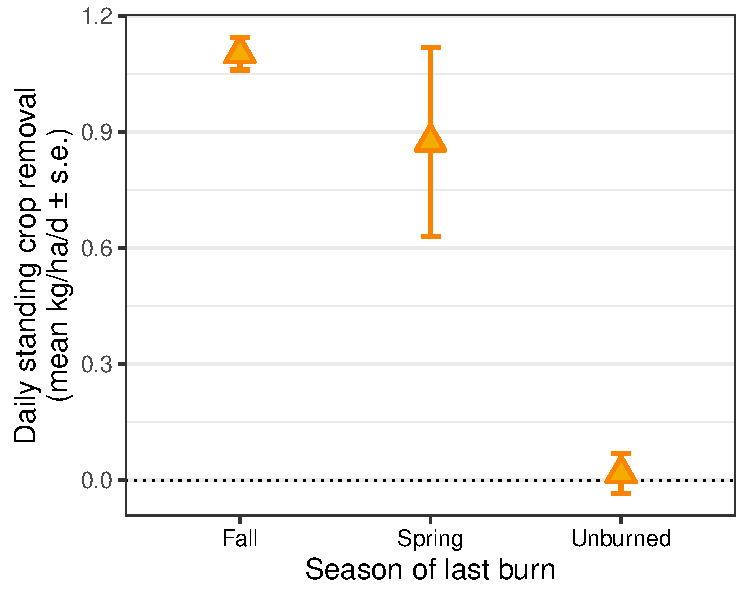
\includegraphics{removal_gg-1.pdf}
\caption{Mean differences in standing crop between grasshopper exclosures and control frames in plots with three different fire treatments. 
Standing crop was determined by clipping at the end of the four-week study period and differences attributable to grasshopper removal are expressed as mean kg per ha per day.}
\label{removal} % Fig.~\ref{removal}
\end{figure}

Standing crop was statistically-significantly lower outside of grasshopper exclosures in both fall and spring burns (\(t =\) -7.6,
\(P\) \textless{} 0.001 and \(t =\) -6, \(P\) \textless{} 0.001, respectively). 
There was no difference in offtake among spring and fall burns (\(P\) \textgreater{} 0.05), with grasshoppers removing approximately 1.0 ($\pm$ 0.2) kg ha\textsuperscript{-1} d\textsuperscript{-1} in each (Fig.~\ref{removal}). 
Standing crop was not different between grasshopper exclosures and areas accessible to grasshoppers in unburned plots (\(t =\) -0.12, \(P\) \textgreater{} 0.05).
 Offtake was significantly lower in unburned plots than plots burned in both the previous fall and spring (\(P\) \textless{} 0.01 and \(P\) = 0.01, respectively).

\begin{figure}
\centering
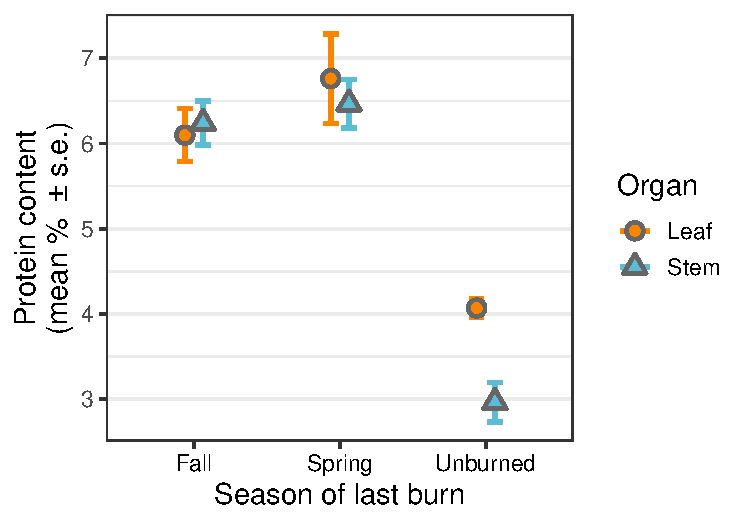
\includegraphics{value_gg-1.pdf}
\caption{Mean protein content of western wheatgrass \emph{Pascopyrum smithii} sampled from three burn treatments as a percentage of total dry matter. 
Red circles indicate the protein content of leaves; blue triangles are stems.}
 \label{value} % (Fig.~\ref{value})
\end{figure}

Crude protein content varied among the fire treatments (\(t =\) 57, \(P\) \textless{} 0.001; (Fig.~\ref{value}). 
Crude protein content in fall and spring burns averaged 6.4\% ± 0.2 s.e. and did not differ among each other (\(P\) \textgreater{} 0.05). 
But crude protein content in unburned  plots was lower than in both fall and spring burns plots (-2.7, \(P\) \textless{} 0.001 and -3.1, \(P\) \textless{} 0.001, respectively).

Across all samples, crude protein content did not vary among leaves and
stems (\(t =\) 2.7, \(P\) \textgreater{} 0.05). Despite a trend towards
higher crude protein in leaf tissue in unburned plots (Fig.~\ref{value}), the
pattern was not influential enough to create a significant fire
treatment \(\times\) organ interaction (\(t =\) 2.1, \(P\)
\textgreater{} 0.05).

\begin{figure}
\centering
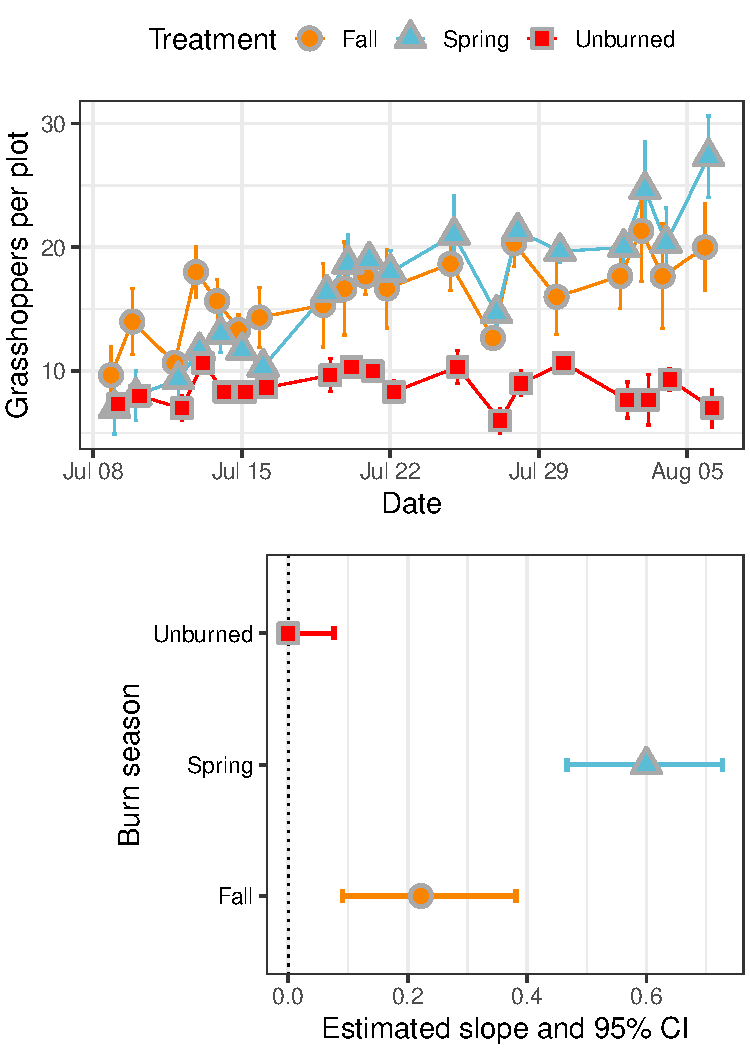
\includegraphics{tau_gg-1.pdf}
\caption{Observed grasshopper counts per square meter. 
Red indicates data taken from fall burn treatments, green from spring burn treatments, and blue from unburned (control) plots.
\emph{Bottom} shows data from Kendall's Tau statistic which assessed the observed count trendline consistency over time. 
Our tau values were compared against the null hypothesis that there was no trend in our data. 
95\% confidence intervals were calculated to show the possible variance in slope for the data over time. 
Most grasshoppers observed were the migratory grasshopper \emph{Melanoplus sanguinipes}.}
\label{tau} % Fig.~\ref{tau}
\end{figure}

Grasshopper abundance was similar across plots at the beginning of the study period (early July) but increased significantly over the next month in fall and spring burn plots (\(\tau =\) 0.29, \(P\) \textless{} 0.01 and \(\tau =\) 0.62, \(P\) \textless{} 0.001; Fig.~\ref{tau}). 
Grasshopper abundance remained constant over the study period in unburned plots (\(\tau =\) 0.039, \(P\) \textgreater{} 0.05). 
While grasshopper abundance increased in both burn treatments, the rate of increase was approximately three times greater in plots that had been most recently burned in the spring than those that had been burned in the previous fall (Fig.~\ref{tau}, \emph{bottom}), which represented more than a five-fold increase in density from approximately 10 to 55 grasshoppers m\textsuperscript{-2} (Fig.~\ref{tau}, \emph{top}).

\section{Discussion}

Previous research indicates that prescribed fire reduces grasshopper
density \citep{joern2004, vermeire2004}, our study, however, saw
heightened density in small patch burning treatments which could have
massive implications for predicting rangeland herbivore competition.
Fire as a method of control varies greatly in effectiveness from species
to species; certain species, such as Hesperotettix viridis, can be
reduced by as much as 88\% \citep{vermeire2004}. Flightless species of
grasshopper and species that are heavily reliant on specific plant hosts
are especially susceptible to fire disturbances \citep{matenaar2014}.
Thanks to nutrient buffering produced by fire treatment
\citep{spiess2020}, protein availability produced a magnet effect which
we believe caused the heightened density and offtake in burned plots
\citep{meyer2002}. These findings indicate fire disturbance can produce
pockets of extreme competition between range herbivores, with much less
forage for ungulates than what is seemingly available.

The dominant grasshopper at our study area, the migratory grasshopper \emph{Melanoplus sanguinipes}, is frequently responsible for the largest outbreaks, making it especially damaging to farmers and ranchers throughout the Great Plains \citep{onsager2000, olfert2021}.
M. sanguinipes' preferred diet is a nitrogen and carbohydrate ratio of
1:1, making them especially robust and better able to adapt to
nutritionally variable seasons \citep{behmer2008}. Furthermore, these
grasshoppers have the fastest egg production rate at intermediate
dietary nitrogen levels of around 4\% \citep{joern1998} and use nitrogen
to maintain their health and function \citep{schmitz2010}. Due to their
robust qualities, these grasshoppers were incredibly abundant on the
Northern Great Plains in the summer of 2021. Although our burned plots
had higher nitrogen than what is ideal for egg production, the
competition between grasshoppers and the overall low nitrogen content of
the landscape pushed M. sanguinipes to our plots to supplement their
diets. Primary productivity in the Northern Great Plains is directly
linked to rainfall \citep{padbury2002}, therefore the steady increase in
grasshopper density on our burn treatment plots is most likely
attributable to an intensification of the magnet effect as the summer
long drought progressed given that emergence typically peaks in late
June \citep{belovsky1995, humphreys2022}. While other research suggests
that grasshoppers can be attracted to heterogeneous areas for
thermoregulatory microhabitats \citep{joern2013}, the rapid increase in
grasshopper density and the worsening of the drought over the summer
points to a nutrient pull rather than a beneficial microhabitat. High
temperatures, which we experienced consistently throughout the summer
heat wave, weaken M. sanguinipes ability to fight infection
\citep{srygley2022}, further indicating that these grasshoppers are
drawn by nitrogen content and not thermoregulation when shade was nearly
completely absent in the burned plots.

Our study differs from other pyric herbivory studies because it was
conducted with small, clustered areas of burn. Because density increased
so greatly with burn in this study, it indicates a need for further
research into small burn resource utilization by range grasshoppers.
Future directions for our study can examine how grasshopper density
changes with distance from a burn edge for a large burn area. This
information could provide a clearer picture of recolonization effects
created by burn scars combined with magnet effects. Recolonization
presents an avenue for this research to be applied to larger burns in
the Great Plains region, which are becoming more and more common.
Grasshopper density changes could also be further examined through the
offtake rate over time. Further research is needed to see if the offtake
rate increased in burned plots over the duration of the drought. This
would show that offtake is directly related to the quality of the
surrounding forage. Because climate change is intensifying drought
conditions \citep{derner2018}, understanding how offtake will change
will better inform ranching practices to ensure sustainable competition
between grasshoppers and livestock.

Our study has important implications for ranch practices in the Northern
Great Plains. Because prescribed fire is so often used as a forage
buffer for cattle ranching \citep{spiess2020}, it is important to know
how much of the available forage will go to cattle and how much will be
consumed by grasshoppers. Our research already goes against the
population dynamics between grasshoppers and prescribed previously
described \citep{joern2004, vermeire2004}, so it is very likely that
grasshopper abundances are being underestimated when determining how
many cattle can be put out to pasture without overgrazing the landscape.
Furthermore, because the density changed so much over the course of the
study, ranchers must reevaluate the level of competition at the
beginning of the season compared to the end of the season when resources
are even more scarce in a drought.

\backmatter


\bmhead{Acknowledgments}

We appreciate the assistance of Cheryl Murphy, with protein analysis at LARRL, and Nichole Davis, with grasshopper identification at NPARL. 


\bmhead{Conflict of Interest} 

The authors declare that they have no conflict of interest.

\bmhead{Funding} 

NGH received salary support from the USDA-ARS Plains Area co-funded internship with matching funds from LARRL and NPARL. 

\bmhead{Ethics statement} 

This article does not contain any studies with human participants or animals performed by any of the authors.  

\bibliography{HopperzBib.bib}

\end{linenumbers}
\end{document}
